\documentclass[10pt,a4paper]{report}
\usepackage[latin1]{inputenc}
\usepackage{graphicx}
\usepackage{listings}
\lstset{language=C}
\begin{document}

\tableofcontents

\chapter{The Project}

\section{Outline}
\subsection{What it is}
Altitude is our reversible interpreter for the C programming language. The goal of the project is to build a teaching environment which will provide a safety net for C programmers, consisting of a minimal development environment with extensive debugging support. The various nooks and crannies of C are hard to learn for a novice programmer.

When we say it is reversible, we mean that unlike traditional debuggers, where one starts the program, runs the code forward until a problem is hit, or particular conditions met (breakpoints, for example) then looks at what is wrong, it is possible to run the program backwards until similar conditions are met, and see where things went wrong, and what caused them to do so.

C compilers usually focus on producing the fastest correct code possible and indeed, many programmers chose to use C because of its speed advantage over other languages. This focus on speed combined with the internal architecture of physical computers means that the compiler is limited in what data it can put in an executable. Our debugger is based around a virtual machine that runs C code keeping much more metadata than is usual, since we want to focus on code correctness, not speed. This means we can detect a wide variety of errors which, although they affect C code compiled and run everywhere, a normal compiler cannot prevent and a normal dynamic analysis tool cannot report in detail, only detect.

\subsection{Why is it useful}
This project aims to prevent a significant amount of bugs derived from a novice's lack of in-depth understanding of how C works. There are many cases where even experienced users are driven to frustration by subtle differences in how code is handled, and nobody should have to know exactly how every compiler their program may ever be run on will handle their code. To this end, our aims are to prevent implementation-specific code from being written, and to provide reasons why any given error is, in fact, an error.

\section{Structure}
This project was envisioned as a chain of tools which could be developed separately. The core components are a compiler from plain C code to an s-expression based format which encodes location information, an assembler/disassembler which loads this s-expression format and compiles it to bytecode (and vice versa), and a virtual machine, which executes the bytecode. This forms a command line toolchain, which accepts a command language of our own devising. The GUI interacts with an instance of this toolchain via the command language using standard input and output.

\subsection{Reversible Virtual Machine}
The core component of the system, this actually runs any given program, and produces debugging output. The virtual machine design includes some innovations, not the least of which is the elegant patch model of execution described in later sections, which enables the reversible operation of the system. The virtual machine runs the result of compiling and assembling C code, but unlike traditional compilation processes, large amounts of information about the source is retained, since we are focusing not on speed of operation but on completeness of information when the inevitable errors occur. The VM is written largely in C with some C Pre-Processor. The VM may be found in the vm directory in the project source. It's invoked with the command line "altitude filename" where filename is the location of some input C source. This is actually a script which compiles the C source passed into s-expression before invoking the actual program to be run, \lstinline{altitude_bin} on the resulting .sexp file.

\subsection{Compiler}
This component processes the raw input C code and runs it through the C Intermediate Language library, which is written in OCaml. This greatly simplifies the syntax of the program, replacing various compound constructs with simpler ones wherever possible and reducing the syntax used in the program to a small set of operations which are sufficient to express the semantics contained within. This simplified C is then processed again to strip from it information about the location of source items, and this results in C code expressed in an s-expression based format. The CIL powered compiler is to be found in the cilcomp directory in the project source. It's invoked with the commandline "ccomp filename", where filename is the name of the input C source.

\subsection{Assembler/Disassembler}
The assembler is not a discrete program, but rather a library which is used to convert a sexpcode program into VM-executable form. This library consists mainly of a means of defining bytecodes, mapping them to actual instructions expressed in C code, and associating names, types and s-expression tags with them, all of which are used throughout the system to propagate information about the code being run.

\subsection{GUI}
The Graphical User Interface (GUI) for Altitude allows the end user to easily interact with the VM. There is a fairly simple protocol that the VM respects; the GUI uses this protocol to communicate with the VM. The GUI is styled after common integrated development environments, such as Eclipse or Netbeans. It's written in \lstinline{C#} using the .Net framework, and runs equally well on both Windows and Linux under the Mono project's .Net implementation

\section{Completion}
We have not finished the project in it's entirety as laid out in the initial design and specification documents, but a sizeable portion of it is done. The system can execute and report errors in C code, so the core functionality is there. Not all of C is yet supported, however, this is only a matter of time. There follows a list of the major features we have completed.
\begin{itemize}
\item Compiler from C to simplified C syntax
\item Assembler/Disassembler from simplified C to VM Bytecode
\item VM runs but not all instructions are implemented
\item GUI sufficiently complete to allow users to view, run and diagnose problems with C programs the VM can run
\end{itemize}

\section{Future Work}
There is of course much future work that can be done on this project. Some of the things we'd like to do are listed below.
\begin{itemize}
\item Patch model of execution not implemented due to time constraints
\item GUI has scope for improvement, as with all user interfaces
\item System should be able to self-host
\item Implementation of all of C99 as per the standard
\item Ability to link against external C libraries to allow for running of user code without needing to sandbox the entire codebase
\end{itemize}

\chapter{Technical Documentation}
\section{Altitude Virtual Machine}

\subsection{Definitions}
"Userspace" and "user objects" refers to objects in the program being run under Altitude (the user program), so, for instance, user source code is the source code of the user program, a user type is a type used in the user program (which often won't exist in Altitude's source), a user int is an int as defined in the user program (in physical memory, it may not be represented as an "int" in Altitude. Altitude enforces that user ints are 32-bit signed, no matter what the size of an int on the platform altitude is compiled).

"System" is the opposite, and refers to things defined in Altitude's source. For instance, user ints aren't necessarily represented as system ints. A system call is a call made in user code to a function defined internally to Altitude, not in user code. For instance, user-space "malloc" is a system call.

The "program" is all of the parts of the user program that are known at compile time and don't change. For instance, functions (and their code), types, global variables (their declarations and initialisers but not necessarily their runtime values) are part of the program.

A "location" is a reference to user source. It contains a filename, line number, byte position in the file, and reference to the enclosing function. Any subset of these may be present (e.g. sometimes it's difficult or impossible to give an exact line number, sometimes things happen outside any function, etc.).

A "blob" is a piece of memory guaranteed to be contiguous by C. The C standard generally refers to these as "objects", but we've chosen the term "blob" as it's less confusing to those who are used to object-oriented programming (For instance, OO programmers might consider each element of an array an "object", while the entire array is one "blob" in Altitude). Local, global and function-static variables each have a single associated blob, and new blobs can be created at any time by a call to "malloc".

"Sexpcode" is the s-expression-based, Lisp-like form of a C program that the VM receives from the Altitude compiler. A "sexp", is a single, possibly nested, s-expression as used to build sexpcode.

A "stack frame" of a user-function is the activation record for that function and contains the values of the functions formal arguments and local variables. The name "stack frame" is chosen to be consistent with other systems, in Altitude they aren't actually stored on a physical memory stack.

When this document speaks about "types", or "the type system", it is talking not about the C type system, but the Altitude one. These differ in a number of small, mostly irrelevant ways. Generally, the differences are that C defines some types to be different but compatible, while Altitude collapses these definitions into one. For instance, a function argument of type int[10] is just passed as a pointer in C, and it is legal to pass to a function that requires an int[10] an int[15] (or even an int[5], although that often causes bad things). In Altitude, there are no array types in function parameters, just pointers. Another difference is that Altitude conflates "signed char" and plain "char", which is not the case in C (C says "char" is a distinct type from both signed and unsigned char, but must be completely equivalent to an implementation-specified one of them. Yippee.).


\subsection{VM Structure}
Structurally this VM is a stack machine. The is a ``stack'', which is used to store all of the intermediate values of a computation. For instance, the complex expression 2 + (5 * 7) compiles down into the sequence of instructions ``push 2 onto the stack, push 5, push 7, multiply the top 2 and push the result, add the top 2 and push the result''. For access to memory, there are also instructions to push local or global variables onto the stack, and to manipulate pointers.

The stack is typed, and many operations have built-in sanity checks, for instance, Altitude will check for overflow whenever two integers (of any integer type) are added.

\subsubsection{Use of Pointers}
In this VM, pointers are used heavily as a means of abstraction. Pointers are explained in detail in later sections of this document, so for now it will suffice to say that in Altitude, what corresponds to a pointer in the context of the user's program has lots of metadata associated with it in the VM to effectively diagnose problems. Pointers are used to abstract upon fundamental operations, since a lot of such operations fit nicely into a model where a pointer is pushed onto the stack, and an operation is performed upon it. Since we had to implement pointers for the rest of C, we decided to use them as much as we could to reduce the cost of implementing them, and found that we got lots of behaviour that would otherwise have had to have been special-cased out for free!

For example, to call a function, the VM pushes a pointer to that function onto the stack, and then calls the function through the pointer. This means that function pointers in C can be expressed directly in terms of VM-level pointers, since the mechanism is the same in both contexts. Pointers are also used for local variable access: a pointer to the variable in question is pushed onto the stack and dereferenced to obtain the value of the variable. All operations on that variable in user code become operations on a VM-pointer to the variable when compiled into bytecode. Of course, the VM's pointer implementation is used to represent plain old C pointers as well.

Altitude has no instructions to read or write to a local variable, you simply load the address of it (as a pointer), and then you can use the standard pointer instructions to dereference it or assign through it.

\subsection{Journey of a Program}

By the time the VM gets a user program, it has already been compiled into sexpcode. The level of abstraction of sexpcode is like a type-aware assembly language. For instance, loops and if statements have been compiled away to explicit "goto"s, but operations like sizeof and finding a field of a structure given a pointer are left in symbolic form, and haven't been compiled down to constants or pointer arithmetic.

Sexpcode has a simple form. Each sexp has a tag, chosen from a fixed set defined by an enum in sexp.h, and any number of children. Each child is either a string, an integer, or a sexp. Children of a sexp are represented as \lstinline{struct sexp_element}, which contains a union tagged with what type of element it is. So, it is common to see code like:

\begin{verbatim}
        if (sexp->nelems == 1 &&
            sexp-elems[0].type == ST_SEXP){
          struct sexp* only_child = sexp->elems[0].data.sexp;
        }
\end{verbatim}

The sexpcode is then passed to the function "compile" (in bytecode.c) which generates a struct program. The top-level objects are types, global variables, and functions. They are processed in that order, as variables may refer to types and functions may refer to either variables or types. "compile" separates out the three categories, then passes the types to \lstinline{build_typemap} (the "typemap" is explained below)


\subsection{Pointers and the Typemap}

To explain some of the oddities of C and how we handle them, I'll refer to Java as an example of a language which is at least superficially similar to C, but does these things differently.

In Java, a pointer (reference) always points to an entire blob (object). You can't point to the "foo" field of an object in Java. (The "foo" field may well be an object reference, but that's entirely different. You can't refer to the "foo" field itself in a way that you keep pointing to it even though it may change). In C, however, anything that you can access (and many things you can't) can be pointed at.

So, a Java reference carries a fixed, small set of assumptions. By having a Java reference, the programmer is assuming that there is an object of the referred-to type beginning at the memory address given by the reference. These are enforced by the implementation with a combination of compile-time typechecking and garbage collection.

A C pointer is entirely different, and the set of assumptions made by the programmer about the pointer is often not completely known at compile-time. First of all, the mere act of having a pointer does not make any assumptions about memory (unlike in Java). It is perfectly OK in C to have a pointer such as \lstinline{&(((int*)NULL)[5])}, pointing at the 6th element of a null array, about which no assumptions at all can be made.

Rather, the assumptions in C are made by reading from or writing to the memory pointed to by the pointer. The first and most basic assumption made when reading or writing is that the pointer lies within the boundaries of an allocated, un-freed blob (blobs are allocated as part of a function's stack frame or by malloc() and freed upon return or free()). When this assumption is violated, the behaviour is undefined. Typical behaviours are a crash or silent corruption of memory.

Unlike Java, these assumptions are not required to be checked at runtime by the implementation. As with the other assumptions that an implementation need not check, Altitude makes an effort to check it, and report an informative error message if it doesn't hold.

There are various other tools that check this assumption to varying degrees of accuracy, through instrumentation of source code (e.g. GNU gcc's "mudflap") or analysis of dynamically running machine code (e.g. valgrind's "memcheck"). Since these tools operate on compiled code, they often have some information loss. For instance, valgrind can't detect when pointers to stack variables go off the end of their blob and access other stack variables instead, as it just sees the stack as an opaque chunk of memory and sees the invalid access as valid, without realising it's to a different part of the stack.

Still, tools other than Altitude can check this assumption to a high degree of accuracy, without Altitude's performance penalty.

Altitude's power comes from being able to check other, more subtle, assumptions. There are other assumptions in C about memory access. These assumptions have a lesser penalty: when they don't hold, the program may still work and only the value of a particular expression is undefined. A standard example is reading from uninitialised memory (which the likes of valgrind can check), or reading from a piece of memory used as structure padding (which the likes of valgrind can't check). It is incorrect to abandon the execution of a program when one of these assumptions is violated. Theoretically, a C program could create an array, put a valid value in its first element, copy the entire array to a new location (so all but the first element cause reads and writes of undefined values), and then perform some action on the first element.

So, Altitude doesn't cause an error upon such accesses. Instead, if an access is shown to give an undefined result, the value returned is marked as "invalid". Invalidness propagates through the program, and a warning is printed if an invalid value is used for anything suspicious (allocating an invalid amount of memory, outputting and invalid value, dereferencing an invalid pointer, etc). Configurably, the warning may also be printed for every operation involving an invalid value, although this may be a bit extreme as many valid operations can be performed involving some internal manipulation of invalid values (e.g. the array scenario above). As a simple future extension, users will be able to configure this warning level on a per-function basis, to inform Altitude that a given function does something unusual but that the user trusts its implementation.

So, what are these subtle assumptions that Altitude can check but other systems can't?

For these examples, assume the following is defined in user-code:

\begin{verbatim}
  union U{
    int num;
    char* str;
    void* ptr;
  };
  struct S;
  struct S{
    struct S* next;
    int value;
  };

  struct A{
    struct S st;
    union U un;
    char ch;
  };
  struct B{
    struct S st;
    int num;
  };

\end{verbatim}

C makes a number of guarantees about structs and unions. In particular, the first element of a struct is guaranteed to start at the same address as the struct itself, and all elements of the union start at the same address.

Consider an object whose type is "union U". If the "num" element was last assigned to, and the "str" element is read, Altitude will mark the result as invalid. If the "str" element was last assigned to, and the "ptr" element is read, Altitude will *not* mark the result as invalid, as unions are guaranteed to put all elements at the same address and pointers are guaranteed to be convertible to each other without changing the in-memory representation. Likewise, if the ptr element is assigned to, and the str element is read, Altitude will return "ptr" as "str" without complaint, but will maintain the type of "ptr", and will cause an warning if a user accesses the pointer as if it were a string, or passes it to a string-requiring function like strtol.

This example shows that "invalidness" is a deeper concept than one-bit-per-memory-location (as used by tools which detect uninitialised memory accesses), as a given piece of memory can easily be valid as one type and invalid as another.

A more interesting example: suppose a function takes a \lstinline{struct A* pa}. It casts it to a \lstinline{struct B*}, so it now has both \lstinline{pa} and \lstinline{pb} which point to the same location. Further suppose that this piece of memory was previously used to store a \lstinline{struct A}, so all the fields of \lstinline{*pa} are valid (and let's say the union stored an int). Finally, suppose that the blob of memory pointed to by \lstinline{pa} or \lstinline{pb} is big enough to hold either a \lstinline{struct A} or a \lstinline{struct B}.

The function can happily read and write to the fields of \lstinline{*pa}. Furthermore, it can validly read and write to \lstinline{pb->st.next} and \lstinline{pb->st.value}, as \lstinline{pb->st} is guaranteed to be the same as \lstinline{pa->st}. Reading from \lstinline{pb->num} will not necessarily return \lstinline{pa->un.num} as the implementation is allowed to have different amounts of padding between elements of the two structs. The read from \lstinline{pb->num} won't crash the program, but may produce an invalid value.

Suppose then, that the function passes \lstinline{&pb->num} to another function. This other function gets an \lstinline{int*} argument, called i. Reading from \lstinline{*i} will succeed but produce an invalid value for the reasons above. Writing to \lstinline{*i} will have a very interesting effect: it will succeed, but it will invalidate \lstinline{pa->un} and \lstinline{pa->ch}!

This is because the program can't rely on a particular layout of structures (it is chosen arbitrarily by the compiler, with certain restrictions). So, it is possible that in a conforming C implementation, the write to \lstinline{*i} will overwrite all or part of \lstinline{pa->un} or even all or part of \lstinline{pa->ch}! (Unusual layouts like these can happen if a compiler sees two similar structures and decides to pack one tightly for optimal space usage, and pad one generously to aligned boundaries for optimal speed). Altitude will detect that the write to \lstinline{*i} invalidated \lstinline{pa->ch} even though, in Altitude's layout, the objects don't overlap.

In C, a write to a memory location can invalidate the contents of an entirely different memory location (simply because the program couldn't possibly have known the locations were non-overlapping when the programmer wrote it), and Altitude can detect this sort of bug even though the invalidated memory location is not changed by the invalidating write!

As it happens, \lstinline{pa->ch} won't be changed by the write since Altitude lays out \lstinline{pa->ch} after the address pointed to by \lstinline{pb->num}, but Altitude can also detect that it is possible for a conforming implementation of C to overlap them, and so invalidates \lstinline{pa->ch}.

This is what makes pointers in Altitude interesting: they carry information not just about what they point to, but what could be affected by a write through them (which may be much larger than their target). Messages are generated not only from inconsistencies in the program, but also from conditions that could cause inconsistencies in alternative implementations of C.

To bring it back to the Java comparison: the int pointer i has more built-in assumptions than "there is an int at this memory address". It contains assumptions about the layout of memory around the int ("there is a struct B containing this memory address"). The assumptions for a particular pointer don't hold consistently, as in Java. It is merely required that for any set of assumptions active during a memory read, the last write to that piece of memory was working under the same assumptions.

\subsection{Patches and Reversibility}
Patches are a concept we use to model the execution of C programs. It is the patch model that allows reversibility to be so easily implemented on our virtual machine.

The state of the VM is all the information pertaining to the running program, such as the call stack, values of the local variables, values of global variables, and any data allocated on the heap.

We need to be able to switch from state to state while still maintaining enough information to go back to earlier ones. One point to note is that we needn't store every state, it is possible to just store states every so often as if we can restore an early state we can run forward from that point to get later ones.

We can store this information as a series of patches. A patch from state s1 to s2 is enough information such that, given all the information we have at state s1, we could build state s2, and given the information at state s2 we could build s1.

A patch could be represented as "From s1 to s2, these variables were changed from "some values" to "some other values", "these bits of memory" were allocated and had "these bits of data" stored in them, "these bits of memory" were freed and had "these bits of data" at the time they were freed".

The point here is, a patch from s1 to s2 only stores the data that changed between states s1 and s2. This means we can run the VM in a reasonable amount of ram.

Patches, as described, have some interesting structure. Firstly, consider merging two patches. If we have two patches to the program state which come one after the other, we can merge them into one big patch from the original state into the newest one.

Secondly, consider the null patch. That is, the patch which says "nothing changed". Now consider the initial state, that is, the state of the VM just upon entry to main(). This will be referred to as the "base state". The state of the program can be considered as a big patch against the base state. This is not just an idle observation, it means we can actually store the current state of the running program as just another patch, and we need no special data structures for it.

Suppose we want to save a checkpoint to return to during the running of the program (it doesn't really matter where we do this, every N instructions would be reasonable). We can take the patch representing the current state, add it to a list of checkpoints, and set our "current state" patch to the null patch (it is now a patch against the most recently saved checkpoint). Thus, saving snapshots can be done really quickly.

That works fine for writes, but for reads we're going to need to know the current value of the variables. If we just have access to a list of differences from the previous state, we'd have to work backwards through the checkpoint list to get the actual value of the variable. So, in parallel we maintain another "current state" patch, representing the current state of all the program's variables. We should maintain the property that merging the checkpoint list yields the current state (i.e. following the history from the beginning will leave us where we are now).

Stepping backward means reversing some checkpoint patches, stepping forwards means applying them again. With some relatively simple algorithms, we can get a lot of behaviour "for free".

\subsection{Merging patches}
One necessary part is an algorithm to merge patches. Here's a rough pseudo-pseudo-code version of it:

Patches consist of a set of variables, saying for each variable whether it was created (allocated) by this patch, destroyed (freed), or changed value.

To merge two patches p1 and p2, then for each variable in either p1 or p2:

\begin{enumerate}
\item If it only appears in p1 or p2, then it should appear like that in the merged patch.
\item If it was created in p1 and modified in p2, then it should appear as created, with the modified value, in the merged patch.
\item If it was modified in p1 and destroyed in p2, then it should appear as destroyed, with the old value, in the merged patch.
\item If it was modified in p1 and modified in p2, then it should appear as modified, from the oldest to the newest value, in the merged patch. 
\end{enumerate}

The other cases are impossible (can't be modified before being created, etc). 

\subsection{Patch Summary}
A brief summary then: a patch in the context of the virtual machine is a difference between two states of the program. A state of the program includes things like the call stack and the local and global variables visible at a given time. Patches are bi-directional, which means you can utilise the same patch to go from a notional state one to state two and also to go from state two to state one. Execution of a program then can be viewed as a long string of patch applications, to get from the initial empty state to the end state. 

One of the most useful and brilliant things about patches is that because they represent differences they can can be merged together to form a larger patch, still going between two notional states, but this time, those states are not adjacent in the actual execution of the program. This built-in compression of sorts is very useful, because, for example, you might not want to keep patches for each recursive step of a heavily recursive function, which might make thousands of recursive calls, but you do want to be able to step back over the computation. It's possible to simply merge each patch created as a recursive call executes with the patch taken as the function is first called, and you'll have a patch that goes straight from function call to result.

Some interesting relationships fall out of this model of execution, namely: patches form a group, in the abstract algebraic sense. We have an associative operation (merging), an identity (the null patch), and an inverse (reversing the patch).

\section{User Standard Library}
No implementation of C is complete without a standard library implementation to accompany it, providing functions for input and output, manipulation and allocation of memory and so on. However, in the case of C code running under Altitude, calls to standard library functions must be processed on a virtual machine, so we must re-engineer parts of it to operate on our stack machine. Functions such as memory allocation and deallocation, for example, must be written by the implementor of the standard library for each machine it will be used on, since any given machine may differ substantially from another in how it physically lays out and handles its memory. The standard library contains functions which cannot be implemented in user-space as defined previously, since they communicate with the underlying hardware (or in our case, software) at a level inexpressible in terms of user-space constructs.

\section{CIL Compiler \& S-Expression Intermediate Language}
Our CIL-based compiler transforms input C source into an s-expression based interim representation, where information about the source of the expressions is included with the expressions themselves. There follows a definition of the format of the s-expression based language and an in-depth example of a the compilation and execution of a simple program.

\subsection{S-Expression Format}
C code is loaded into the VM in an s-expression based format. This file and sexp.c define parsing and manipulation functions for Altitude's sexps. The format isn't quite standard Lisp-like sexps.

\subsubsection{Grammar}
A sexp in Altitude looks like this (in approximate EBNF.)
 
\begin{list}{}{}
\item sexp := '(' 
\item ($\langle$location$\rangle$ $\langle$ws$\rangle$)?
\item $\langle$tag$\rangle$
\item ($\langle$ws$\rangle$ ($\langle$sexp$\rangle$ $\vert$ $\langle$string$\rangle$ $\vert$ $\langle$int$\rangle$))*
\item $\langle$ws$\rangle$? ')'
\item
\item location := '@' $\langle$string$\rangle$ ':' $\langle$int$\rangle$ ':' $\langle$int$\rangle$
\item
\item int := [0-9]+ [a decimal non-negative integer, fits in a 64-bit unsigned int]
\item
\item string := a double-quoted string, where backslash is the escape character and double-quote and backslash are escaped.
\item
\item ws := any amount of newline, carriage return, tab or space
\item
\item tag := 'STRUCT' $\vert$ 'UNION' $\vert$ 'LOOP'
\end{list}

So, a sexp is an opening parenthesis, followed by optional location
information, followed by a tag, followed by any number of children
which are each integers, quoted strings or themselves sexps,
followed by a closing parenthesis.

\subsubsection{Location Information}
Location information is of the form: @"somefile.c":20:500 which means character 500 which is on line 20 of the file
"somefile.c". It is optional. This location information, as you will see from the forthcoming examples, is propagated throughtout the lifetime of the program, even making its way into the bytecode representation. This enables us to give errors detailing the line and byte of source that caused the error, not just the state of the machine at the time the error presented itself.

\subsection{Compiling Example}
The following is an example of a simple C program devised for testing and how it is compiled into s-expressions and loaded into the VM. First the C program is loaded from disk.

\subsubsection{The C source}
\begin{verbatim}
struct astruct{
  int thisval;
};

struct somestruct{
  int val;
  struct astruct obj;
};

int sum(int x){
  struct somestruct s;
  s.obj.thisval = 0;
  for (int i=0;i<x;i++){
    s.obj.thisval += i;
  }
  return s.obj.thisval;
}

int main(){
  return sum(40);
}
\end{verbatim}

\subsubsection{Processed source}
This C source is then annotated into the following form.
\begin{verbatim}
# 1 "programs/simple.c"
# 1 "<built-in>"
# 1 "<command-line>"
# 1 "programs/simple.c"
struct astruct{
  int thisval;
};

struct somestruct{
  int val;
  struct astruct obj;
};

int sum(int x){
  struct somestruct s;
  s.obj.thisval = 0;
  for (int i=0;i<x;i++){
    s.obj.thisval += i;
  }
  return s.obj.thisval;
}

int main(){
  return sum(40);
}
\end{verbatim}

\subsubsection{Simplified C form, after CIL first pass}
This is the output of the plain CIL library, which we further process to explicitly encode location information. It can be seen that the CIL library greatly simplifies the input C code to produce a more verbose but syntactically much less complex piece of code. It should be noted that both of these representations are entirely equivalent, and the behaviour of the resulting program will be exactly the same in both cases. The location information here printed is in comments, ignored by C but stripped out by the next pass.

\begin{verbatim}
/* Generated by CIL v. 1.3.6 */
/* print_CIL_Input is true */

#line 1 "simple.c"
struct astruct {
   int thisval ;
};
#line 5 "simple.c"
struct somestruct {
   int val ;
   struct astruct obj ;
};
#line 10 "simple.c"
int sum(int x ) 
{ struct somestruct s ;
  int i ;

  {
#line 12
  s.obj.thisval = 0;
#line 13
  i = 0;
#line 13
  while (1) {
#line 13
    if (i < x) {

    } else {
#line 13
      break;
    }
#line 14
    s.obj.thisval += i;
#line 13
    i += 1;
  }
#line 16
  return (s.obj.thisval);
}
}
#line 19 "simple.c"
int main(void) 
{ int tmp ;

  {
#line 20
  tmp = sum(40);
#line 20
  return (tmp);
}
}
\end{verbatim}

\subsubsection{In S-Expression form for the VM loader}
Here is the previous program compiled into s-expression form. You can see that the location information has been explicitly encoded as part of each action in the C source.

\begin{verbatim}
(program 
(@"simple.c":1:0 struct
  "struct astruct" (fields (field (type (int)) "thisval")))
(@"simple.c":5:35 struct
  "struct somestruct" (fields (field (type (int)) "val")
                              (field (type (comptype "struct astruct")) "obj")))
(@"simple.c":10:91 function
  "sum"
  (formals (@"simple.c":10:91 var (type (int)) "x"))
  (locals (@"simple.c":10:91 var (type (comptype "struct somestruct")) "s")
          (@"simple.c":10:91 var (type (int)) "i"))
  (body (load_l "s")
        (offset "struct somestruct" "obj")
        (offset "struct astruct" "thisval")
        (constant.int 0)
        (@"simple.c":12:132 assign)
        (load_l "i")
        (constant.int 0)
        (@"simple.c":13:158 assign)
        (label "$LOOPSTART$ALT$0")
        (load_l "i")
        (deref)
        (load_l "x")
        (deref)
        (lt.int)
        (condgoto (label "$ALT$2"))
        (@"simple.c":13:153 goto (label "$LOOPEND$ALT$1"))
        (goto (label "$ALT$3"))
        (label "$ALT$2")

        (label "$ALT$3")
        (load_l "s")
        (offset "struct somestruct" "obj")
        (offset "struct astruct" "thisval")
        (load_l "s")
        (offset "struct somestruct" "obj")
        (offset "struct astruct" "thisval")
        (deref)
        (load_l "i")
        (deref)
        (plus.int)
        (@"simple.c":14:180 assign)
        (load_l "i")
        (load_l "i")
        (deref)
        (constant.int 1)
        (plus.int)
        (@"simple.c":13:158 assign)
        (goto (label "$LOOPSTART$ALT$0"))
        (label "$LOOPEND$ALT$1")
        (load_l "s")
        (offset "struct somestruct" "obj")
        (offset "struct astruct" "thisval")
        (deref)
        (@"simple.c":16:206 return)))
(@"simple.c":19:231 function
  "main"
  (formals)
  (locals (@"simple.c":19:231 var (type (int)) "tmp"))
  (body (load_l "tmp")
        (constant.int 40)
        (load_f "sum")
        (deref)
        (@"simple.c":20:245 callassign 1)
        (load_l "tmp")
        (deref)
        (@"simple.c":20:245 return)))
)
\end{verbatim}

\subsubsection{In literal bytecode form, opcodes mapped to tags for display}
This is the result of loading the previous program into the VM and dumping the result after the bytecode has been generated. For legibilty, the bytecode has a tag associated with each operation, and it is represented here in tag format. Note that even in the bytecode, the location information is still present.

\begin{verbatim}
Global variables:
Function <sum>:
 Arguments:
  signed int x declared in @"simple.c":10:91
 Local variables:
  struct somestruct s declared in @"simple.c":10:91
  signed int i declared in @"simple.c":10:91
 Constants:
  0: signed int =  0
  1: signed int =  0
  2: signed int =  1
 Code:
                                  0000: VAR_LOAD_LOCAL 1
                                  0002: PTR_OFFSET 2
                                  0004: PTR_OFFSET 1
                                  0006: VAR_LOAD_CONSTANT 0
  @"simple.c":12:132              0008: PTR_ASSIGN
                                  0009: VAR_LOAD_LOCAL 2
                                  0011: VAR_LOAD_CONSTANT 1
  @"simple.c":13:158              0013: PTR_ASSIGN
                                  0014: VAR_LOAD_LOCAL 2
                                  0016: PTR_DEREF
                                  0017: VAR_LOAD_LOCAL 0
                                  0019: PTR_DEREF
                                  0020: REL_LT[PS_INT]
                                  0021: GOTO_COND 6 (->27)
  @"simple.c":13:153              0023: GOTO_ALWAYS 33 (->56)
                                  0025: GOTO_ALWAYS 2 (->27)
                                  0027: VAR_LOAD_LOCAL 1
                                  0029: PTR_OFFSET 2
                                  0031: PTR_OFFSET 1
                                  0033: VAR_LOAD_LOCAL 1
                                  0035: PTR_OFFSET 2
                                  0037: PTR_OFFSET 1
                                  0039: PTR_DEREF
                                  0040: VAR_LOAD_LOCAL 2
                                  0042: PTR_DEREF
                                  0043: ARITH_PLUS[PS_INT]
  @"simple.c":14:180              0044: PTR_ASSIGN
                                  0045: VAR_LOAD_LOCAL 2
                                  0047: VAR_LOAD_LOCAL 2
                                  0049: PTR_DEREF
                                  0050: VAR_LOAD_CONSTANT 2
                                  0052: ARITH_PLUS[PS_INT]
  @"simple.c":13:158              0053: PTR_ASSIGN
                                  0054: GOTO_ALWAYS 65496 (->14)
                                  0056: VAR_LOAD_LOCAL 1
                                  0058: PTR_OFFSET 2
                                  0060: PTR_OFFSET 1
                                  0062: PTR_DEREF
  @"simple.c":16:206              0063: FUNC_RETURN
                                  0064: FUNC_RETURN_NONE
Function <main>:
 Arguments:
 Local variables:
  signed int tmp declared in @"simple.c":19:231
 Constants:
  0: signed int =  40
 Code:
                                  0000: VAR_LOAD_LOCAL 0
                                  0002: VAR_LOAD_CONSTANT 0
                                  0004: VAR_LOAD_FUNC 0
                                  0006: PTR_DEREF
  @"simple.c":20:245              0007: FUNC_CALL 1
                                  0009: VAR_LOAD_LOCAL 0
                                  0011: PTR_DEREF
  @"simple.c":20:245              0012: FUNC_RETURN
                                  0013: FUNC_RETURN_NONE
\end{verbatim}

\section{Altitude User Interface}

\subsection{Description}
The GUI was originally to be written in C using Glade to design it graphically, but due to time constraints, we chose \lstinline{C#} for its quick turn-around time and cross platform availability (via the Mono implementation of the .NET Framework). The GUI was designed in Visual Studio 2008, which lead to one or two bugs when run under Linux (end of line being return newline versus newline, for example), but ultimately it runs cleanly on all common desktop platforms. When the GUI is loaded, it opens the main editor form, and the Error and IO Console toolboxes.

\subsection{Implementation}
When the VM wishes to raise an event with the GUI, it writes the following to standard output:

[ERR\_NO] ERR\_MSG

Error number is a defined as an enum; each type of error altitude can check for is given its own number, as are certain special messages to the GUI (not strictly errors). These include when the user program wishes to output data to the IO console. The GUI will colour-code the entries to the error console, based on severity. We also had thoughts about setting the GUI to ignore certain ranges of errors on the fly -  for example, if you knew your program had several errors of type X but only wanted to root out error type Y - but this has yet to be implemented.

The message may contain line number information in the form \lstinline{@file_name:line_no:byte_offset}. The file location metadata is passed through the compilation process in the bytecode. This is then available in the form of a \lstinline{struct location} for the VM to output. The GUI parses the input line for such location information and displays it in the error console. The GUI will also colour-code the entries to the error console, based on severity.

\subsection{UI-VM Command Protocol}
The following is the protocol used by the UI when interacting with the VM. All commands and data are passed between the processes on stdin/stdout.
\subsubsection{Startup}
User starts by selecting a C source code file. This file is passed to altitude as an argument:

UI 'exec's a new process: "altitude code/test/test.c"

At this point, altitude should parse/convert to bytecode and sit and wait - we want to set breakpoints etc. before running the code.

\subsubsection{Commands}

When we want to run forward to the next breakpoint, we send 'run'

[UI $\rangle\rangle$ Altitude] run

When we want to run backwards to the prvious breakpoint, we 'runback'

[UI $\rangle\rangle$ Altitude] runback

When we want to set a breakpoint, we use 'set' followed by a line number

[UI $\rangle\rangle$ Altitude] set LINENO

Similar to unset a breakpoint

[UI $\rangle\rangle$ Altitude] unset LINENO

To reset the program, i.e. jump to the start and wait, we use 'restart'

[UI $\rangle\rangle$ Altitude] restart

To get a dump of variables in scope, we use 'view'

[UI $\rangle\rangle$ Altitude] view

This should return variable list in the following format
\begin{itemize}
\item varlist = var [newline var]
\item newline = newline, return or return-newline
\item var = primtype varname value
\item primtype = char  int ... any of the other variations of integer types
\item value = any single char for a char  any integer for an int (or one of the variations)
\end{itemize}

\subsubsection{Errors and Warnings}

Errors and warnings are passed from altitude on stderr.

They take the form:
[Altitude $\rangle\rangle$ UI] [errno] message

message may contain a reference in the form \lstinline{@filename:lineno:byteoffset}


Altitude will display this on its error console, and if it is a crash-worthy error, the program will alert the user explicitly.

\subsubsection{Screenshot of the UI in action}
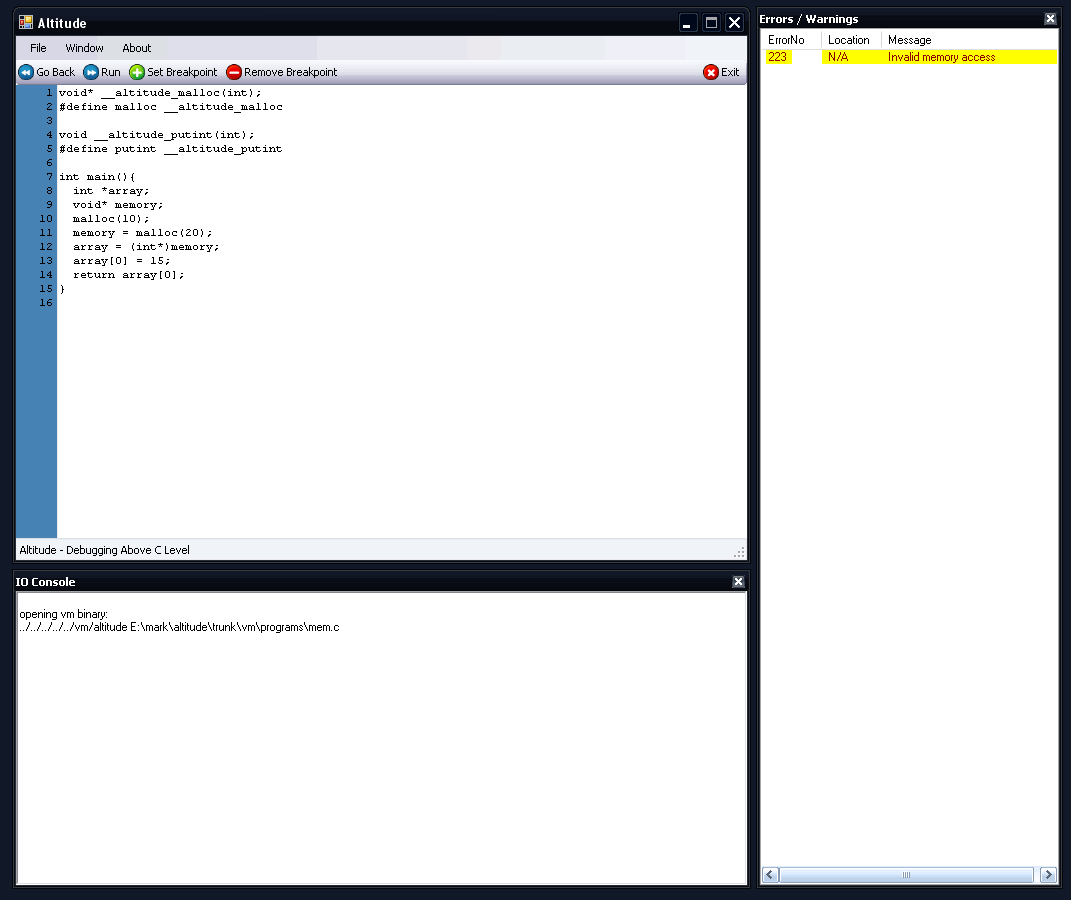
\includegraphics[scale=0.35]{gui_screenshot.png}
\end{document}
